\section{Návrh uživatelského rozhraní - Lo-Fi prototyp}

V poděkování jsem zmiňoval, že při prvotním návrhu UI jsme spolupracovali jako tým v předmětu MI-NUR. V rámci naší semestrální práce jsme navrhovali nový skladový systém vycházející ze Sysla, a zaměřili jsme se pouze na pohled skladníka.\\
První částí návrhu GUI byl mockup, či chcete-li wireframe. Pro jeho tvorbu jsme využili nástroj Axure RP \cite{axure} - jedná se o komplexní nástroj pro tvorbu prototypů, bez nutnosti psaní programového kódu. Lze do něj doinstalovat externí knihovny, které například přidávají hotové designové či funkční prvky a má vlastní řešení kolaborace a verzování ve stylu SVN.\\
Pro naše potřeby jsme tedy do Axure doinstalovali UX Tool Time \cite{uxtooltime}, což je knihovna pro Axure, která nabízí komponenty v \emph{Material designu}. S její pomocí jsme vytvořili návrhy na základní procesy skladníka.\\
Zdrojové kódy tohoto návrhy jsou k dispozici buďto na přiloženém médiu, nebo na webové adrese https://zho703.axshare.com/.\\
Příklad jedné obrazovky - konkrétně naskladnění - vkládám i přímo do textu jako obrázek \ref{picture:axure}. Ještě předtím je ale pro porovnání vložena i ukázka stávajícího skladového systému - taktéž rozpracovaného úkolu naskladnění (obrázek \ref{picture:sysel:naskladneni}).

\begin{figure}[]
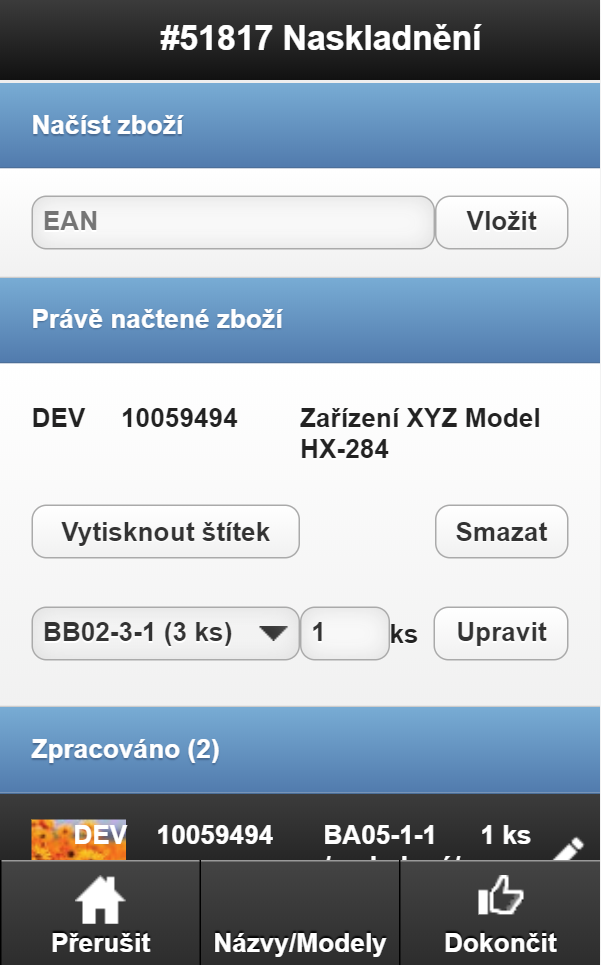
\includegraphics[height=0.6\textheight]{../png/sysel/naskladneni.png}
\caption{Rozhraní skladníka pro naskladňování položek: starý skladový systém} \label{picture:sysel:naskladneni}
\end{figure}

\begin{figure}[]
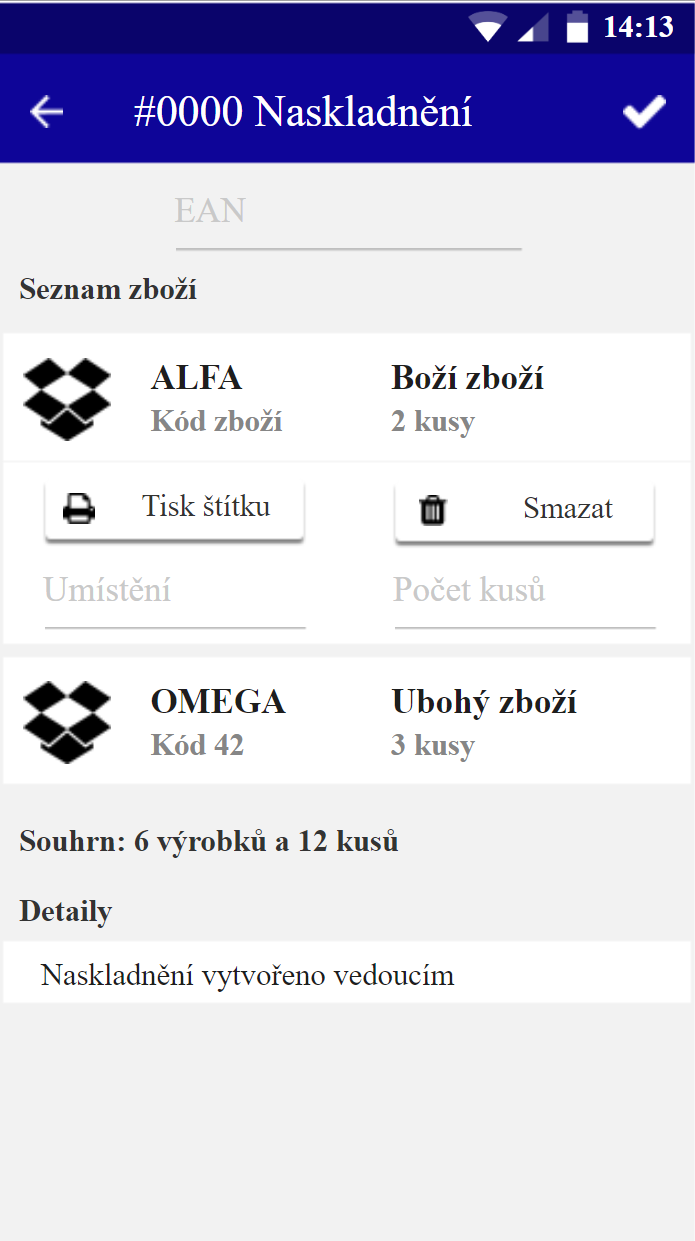
\includegraphics[height=0.6\textheight]{../png/axure/naskladneni.png}
\caption{Rozhraní skladníka pro naskladňování položek: Lo-Fi prototyp} \label{picture:axure}
\end{figure}
